\documentclass[11pt,a4paper]{article}

% ============================================================
% PACKAGES
% ============================================================

\usepackage[utf8]{inputenc}
\usepackage[T1]{fontenc}
\usepackage[margin=1in]{geometry}
\usepackage{helvet}
\renewcommand{\familydefault}{\sfdefault}
\usepackage{microtype}
\usepackage{xcolor}
\usepackage{hyperref}
\usepackage{listings}
\usepackage{booktabs}
\usepackage{array}
\usepackage{tabularx}
\usepackage{tikz}
\usetikzlibrary{shapes.geometric, arrows.meta, positioning, calc}
\usepackage{fancyhdr}
\usepackage{titlesec}
\usepackage{enumitem}
\usepackage{mdframed}
\usepackage{graphicx}
\usepackage{parskip}

% ============================================================
% COLORS
% ============================================================

\definecolor{primaryblue}{RGB}{26, 82, 118}
\definecolor{secondaryblue}{RGB}{41, 128, 185}
\definecolor{darkgray}{RGB}{44, 62, 80}
\definecolor{lightgray}{RGB}{245, 247, 250}
\definecolor{codebg}{RGB}{236, 240, 241}
\definecolor{accentgreen}{RGB}{39, 174, 96}
\definecolor{bordercolor}{RGB}{174, 214, 241}

% ============================================================
% HYPERREF
% ============================================================

\hypersetup{
    colorlinks=true,
    linkcolor=secondaryblue,
    urlcolor=secondaryblue,
    pdftitle={Real-Time Group Chat Application},
    pdfauthor={Ganesh, Venu, Venkat, Dheemanth}
}

% ============================================================
% HEADER & FOOTER
% ============================================================

\pagestyle{fancy}
\fancyhf{}
\lhead{\textcolor{darkgray}{\small Real-Time Group Chat Application}}
\rhead{\textcolor{darkgray}{\small Computer System Design}}
\cfoot{\textcolor{darkgray}{\small \thepage}}
\renewcommand{\headrulewidth}{0.4pt}
\renewcommand{\footrulewidth}{0.4pt}

% ============================================================
% SECTION FORMATTING
% ============================================================

\titleformat{\section}
  {\Large\bfseries\color{primaryblue}}
  {\thesection}{1em}{}[\color{primaryblue}\hrule]
\titlespacing{\section}{0pt}{14pt}{6pt}

\titleformat{\subsection}
  {\large\bfseries\color{secondaryblue}}
  {\thesubsection}{1em}{}
\titlespacing{\subsection}{0pt}{10pt}{4pt}

% ============================================================
% CODE LISTING
% ============================================================

\lstset{
    backgroundcolor=\color{codebg},
    basicstyle=\ttfamily\footnotesize\color{darkgray},
    breaklines=true,
    frame=single,
    framerule=0.4pt,
    rulecolor=\color{bordercolor},
    tabsize=4,
    showstringspaces=false,
    keywordstyle=\color{secondaryblue}\bfseries,
    aboveskip=6pt,
    belowskip=6pt
}

% ============================================================
% DOCUMENT
% ============================================================

\begin{document}

\thispagestyle{empty}

% ------------------------------------------------------------
% TITLE PAGE
% ------------------------------------------------------------

\begin{center}

    \vspace*{1.5cm}

    {\large \bfseries \color{secondaryblue} Course: Computer System Design}

    \vspace{0.5cm}
    \rule{\textwidth}{1.5pt}
    \vspace{0.3cm}

    {\Huge \bfseries \color{primaryblue} Real-Time Group Chat Application}

    \vspace{0.3cm}
    {\large \color{darkgray} Assignment Explanation Report}

    \vspace{0.3cm}
    \rule{\textwidth}{1.5pt}

    \vspace{1cm}

    % ---- Group Members Table ----
    {\large \bfseries \color{darkgray} Group Members}

    \vspace{0.4cm}

    \begin{tabular}{clc}
        \toprule
        \textbf{No.} & \textbf{Username} & \textbf{ID Number} \\
        \midrule
        1 & Ganesh     & 12341080 \\
        2 & Venu       & 12341110 \\
        3 & Venkat     & 12341070 \\
        4 & Dheemanth  & 12341710 \\
        \bottomrule
    \end{tabular}

    \vspace{1cm}

    % ---- Source Code Link ----
    \begin{mdframed}[
        backgroundcolor=lightgray,
        linecolor=secondaryblue,
        linewidth=1.2pt,
        roundcorner=6pt,
        innertopmargin=10pt,
        innerbottommargin=10pt
    ]
        \centering
        \textbf{\color{darkgray} Project Source Code}\\[4pt]
        \url{https://drive/group-chat}
    \end{mdframed}

    \vspace{1.5cm}

\end{center}

\newpage

% ============================================================
% SECTION 1: CLIENT URL & AUTHENTICATION
% ============================================================

\section{Client Access URL}

To access the chat application, open the following URL in a web browser:

\begin{mdframed}[
    backgroundcolor=codebg,
    linecolor=bordercolor,
    linewidth=1pt,
    roundcorner=4pt,
    innertopmargin=8pt,
    innerbottommargin=8pt
]
    \centering
    \textbf{\large \color{primaryblue} \url{http://10.1.75.51:5213}}
\end{mdframed}

\vspace{0.3cm}

When you click the link, the application will open a \textbf{Login Page} that asks for authentication credentials. Use the usernames and passwords listed in the table below to log in.

\vspace{0.3cm}

\begin{center}
\begin{tabular}{clc}
    \toprule
    \textbf{No.} & \textbf{Username} & \textbf{Password} \\
    \midrule
    1 & ganesh     & 12341080 \\
    2 & venu       & 12341110 \\
    3 & venkat     & 12341070 \\
    4 & dheemanth  & 12341710 \\
    \bottomrule
\end{tabular}
\end{center}

\vspace{0.2cm}

\textbf{Note:} Only users in the above list are allowed to access the chat. Incorrect username or password will be rejected by the server.

% ============================================================
% SECTION 2: PROJECT OVERVIEW
% ============================================================

\section{Project Overview}

The \textbf{Real-Time Group Chat Application} is a lightweight real-time communication system built using \textbf{Python WebSockets} on the backend and \textbf{HTML, CSS, and JavaScript} on the frontend.

The system allows the four authorized group members to communicate with each other in real time, through a browser-based chat interface, without requiring any external frameworks.

\subsection{Project Structure}

\begin{lstlisting}
group-chat/
|
|-- server.py        (WebSocket Backend Server)
|-- README.md        (Project Documentation)
|
+-- client/
    |-- index.html   (Login & Chat UI)
    |-- style.css    (Responsive Styling)
    +-- app.js       (Client WebSocket Logic)
\end{lstlisting}

% ============================================================
% SECTION 3: SERVER ARCHITECTURE
% ============================================================

\section{Server Architecture (\texttt{server.py})}

The backend is an \textbf{asynchronous event-driven WebSocket server} built using Python's \texttt{asyncio} engine and the \texttt{websockets} library. It handles all connections, authentication, session state, and message broadcasting.

\subsection{Core Components}

\begin{enumerate}[leftmargin=*, itemsep=4pt]

    \item \textbf{Global Configuration \& State}
    \begin{itemize}[itemsep=2pt]
        \item \texttt{AUTHORIZED\_USERS} --- Dictionary of valid usernames and their access codes (passwords).
        \item \texttt{connected\_users} --- In-memory dictionary mapping active WebSocket connections to user metadata (\texttt{username}, \texttt{ip}).
        \item \texttt{MAX\_USERS} --- Hard limit set to \textbf{4 simultaneous connections}.
        \item \texttt{HOST = "0.0.0.0"}, \texttt{PORT = 4000} --- Server binding address and port.
    \end{itemize}

    \item \textbf{Key Functions \& Coroutines}
    \begin{itemize}[itemsep=2pt]
        \item \texttt{main()} --- Entry point. Initializes \texttt{websockets.serve(chat, HOST, PORT)} and starts the infinite \texttt{asyncio} event loop.
        \item \texttt{chat(websocket)} --- Main per-client coroutine. Handles the full connection lifecycle: authentication check, message reception loop, and disconnection cleanup in the \texttt{finally} block.
        \item \texttt{broadcast(data)} --- Sends a JSON message concurrently to \textbf{all} connected clients using \texttt{asyncio.gather(*..., return\_exceptions=True)}.
        \item \texttt{send\_json(websocket, data)} --- Helper to send a JSON message to a single client.
        \item \texttt{send\_user\_list()} --- Builds and broadcasts the current list of online users to all connected clients.
    \end{itemize}

\end{enumerate}

\subsection{Server Processing Lifecycle}

\begin{center}
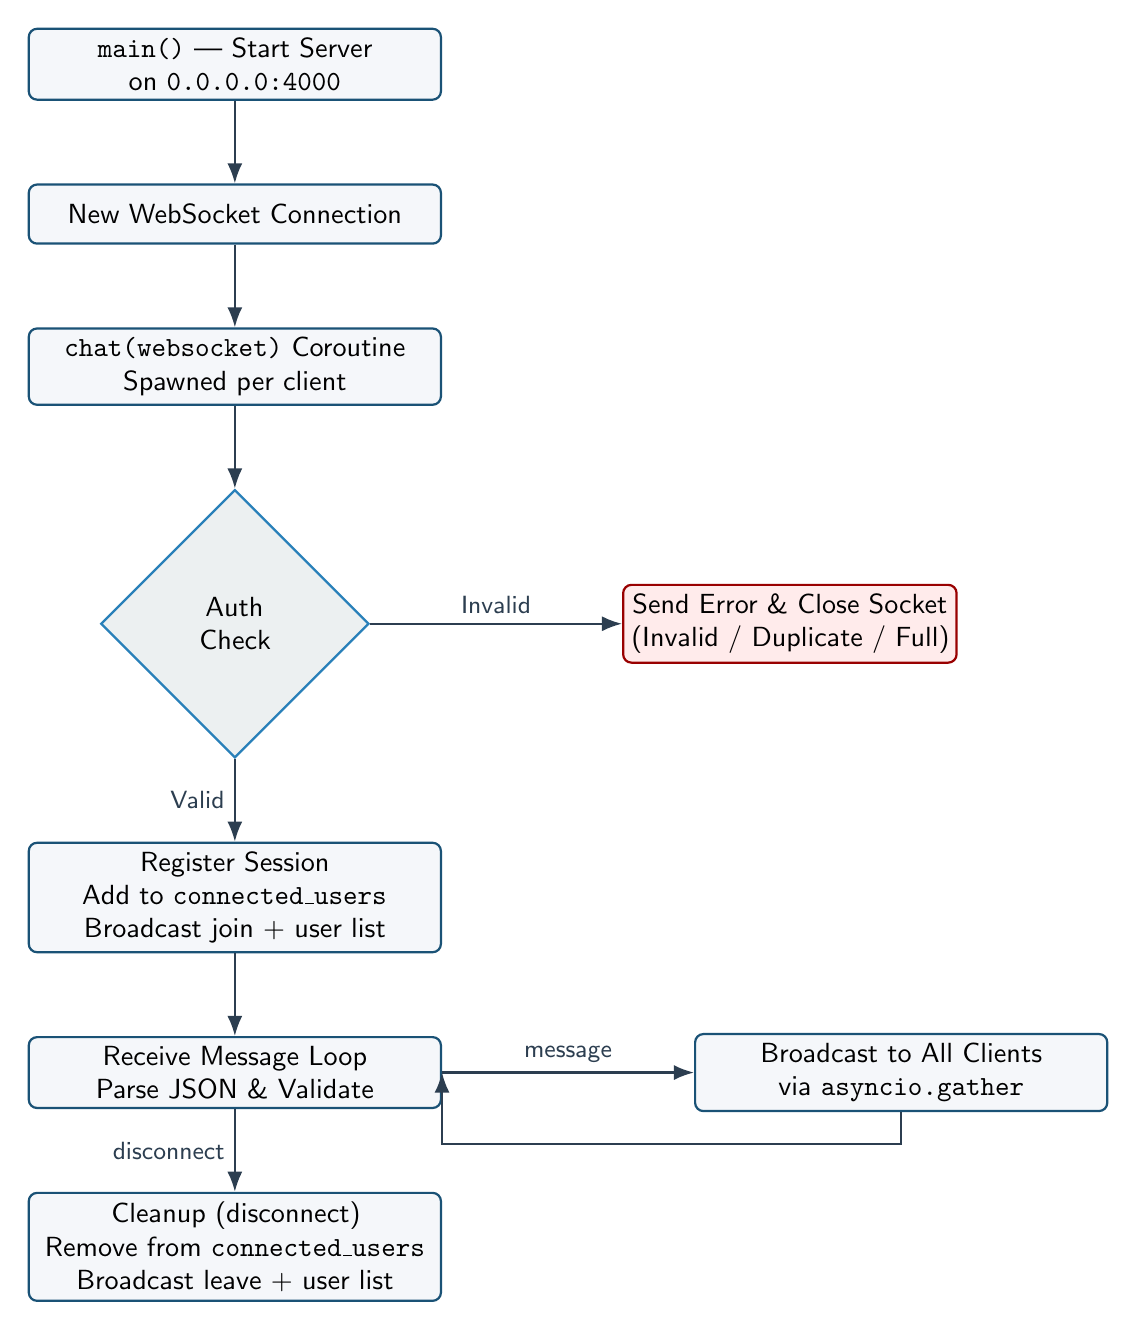
\begin{tikzpicture}[
    node distance=1.05cm,
    block/.style={
        rectangle, draw=primaryblue, fill=lightgray, thick,
        text width=5cm, align=center, rounded corners=3pt, minimum height=0.75cm
    },
    decision/.style={
        diamond, draw=secondaryblue, fill=codebg, thick,
        text width=2.6cm, align=center, inner sep=1pt
    },
    badnode/.style={
        rectangle, draw=red!60!black, fill=red!8, thick,
        text width=4cm, align=center, rounded corners=3pt
    },
    line/.style={draw, -{Latex[scale=1.1]}, thick, color=darkgray}
]
    \node [block]     (main)     {\texttt{main()} --- Start Server\\on \texttt{0.0.0.0:4000}};
    \node [block,     below=of main]  (conn)     {New WebSocket Connection};
    \node [block,     below=of conn]  (chat)     {\texttt{chat(websocket)} Coroutine\\Spawned per client};
    \node [decision,  below=of chat]  (auth)     {Auth\\Check};
    \node [badnode,   right=3.2cm of auth] (reject) {Send Error \& Close Socket\\(Invalid / Duplicate / Full)};
    \node [block,     below=of auth]  (reg)      {Register Session\\Add to \texttt{connected\_users}\\Broadcast join + user list};
    \node [block,     below=of reg]   (loop)     {Receive Message Loop\\Parse JSON \& Validate};
    \node [block,     right=3.2cm of loop] (bcast) {Broadcast to All Clients\\via \texttt{asyncio.gather}};
    \node [block,     below=of loop]  (clean)    {Cleanup (disconnect)\\Remove from \texttt{connected\_users}\\Broadcast leave + user list};

    \path [line] (main)   -- (conn);
    \path [line] (conn)   -- (chat);
    \path [line] (chat)   -- (auth);
    \path [line] (auth.east)  -- node[above, font=\small]{Invalid} (reject.west);
    \path [line] (auth)   -- node[left, font=\small]{Valid} (reg);
    \path [line] (reg)    -- (loop);
    \path [line] (loop.east)  -- node[above, font=\small]{message} (bcast.west);
    \path [line] (bcast.south) -- ++(0,-0.4) -| (loop.east);
    \path [line] (loop)   -- node[left, font=\small]{disconnect} (clean);
\end{tikzpicture}
\end{center}

% ============================================================
% SECTION 4: APPLICATION FLOW
% ============================================================

\section{Application Flow}

The following diagram describes the complete end-to-end flow from the moment a user opens the client URL until they are actively chatting.

\begin{center}
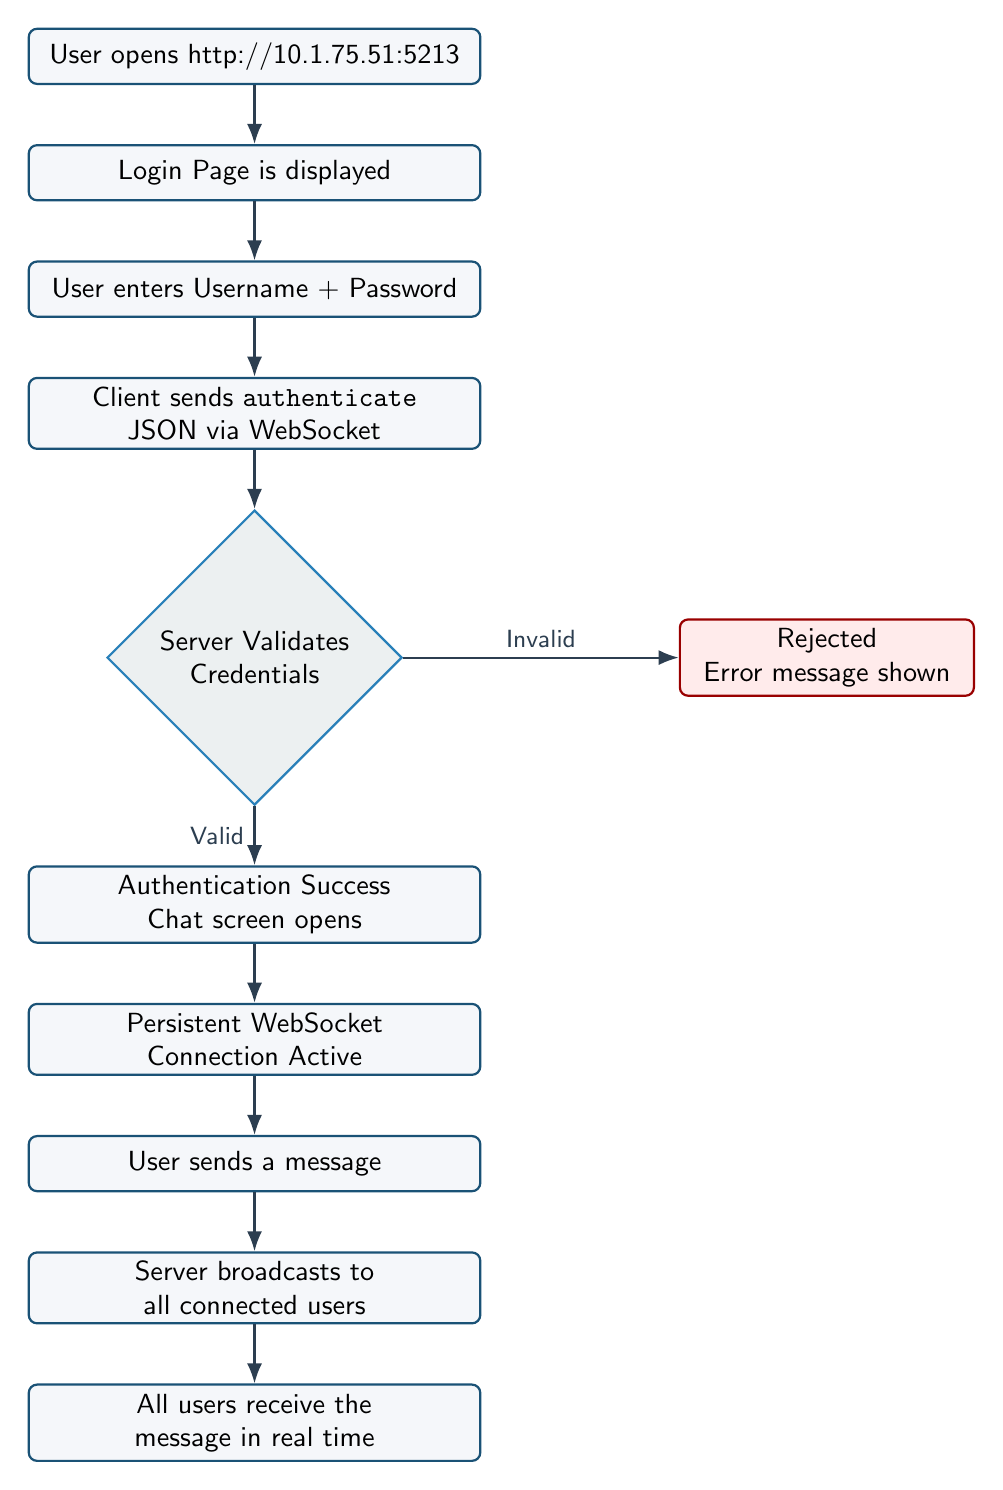
\begin{tikzpicture}[
    node distance=0.75cm,
    block/.style={
        rectangle, draw=primaryblue, fill=lightgray, thick,
        text width=5.5cm, align=center, rounded corners=3pt, minimum height=0.7cm
    },
    decision/.style={
        diamond, draw=secondaryblue, fill=codebg, thick,
        text width=2.8cm, align=center, inner sep=2pt
    },
    bad/.style={
        rectangle, draw=red!60!black, fill=red!8, thick,
        text width=3.5cm, align=center, rounded corners=3pt
    },
    line/.style={draw, -{Latex[scale=1.1]}, thick, color=darkgray}
]
    \node [block]     (open)   {User opens \url{http://10.1.75.51:5213}};
    \node [block,     below=of open]   (login)  {Login Page is displayed};
    \node [block,     below=of login]  (enter)  {User enters Username + Password};
    \node [block,     below=of enter]  (send)   {Client sends \texttt{authenticate} JSON via WebSocket};
    \node [decision,  below=of send]   (check)  {Server Validates Credentials};
    \node [bad,       right=3.5cm of check] (rej) {Rejected\\Error message shown};
    \node [block,     below=of check]  (chat)   {Authentication Success\\Chat screen opens};
    \node [block,     below=of chat]   (ws)     {Persistent WebSocket Connection Active};
    \node [block,     below=of ws]     (msg)    {User sends a message};
    \node [block,     below=of msg]    (bcast)  {Server broadcasts to all connected users};
    \node [block,     below=of bcast]  (recv)   {All users receive the message in real time};

    \path [line] (open)  -- (login);
    \path [line] (login) -- (enter);
    \path [line] (enter) -- (send);
    \path [line] (send)  -- (check);
    \path [line] (check.east) -- node[above, font=\small]{Invalid} (rej.west);
    \path [line] (check) -- node[left, font=\small]{Valid} (chat);
    \path [line] (chat)  -- (ws);
    \path [line] (ws)    -- (msg);
    \path [line] (msg)   -- (bcast);
    \path [line] (bcast) -- (recv);
\end{tikzpicture}
\end{center}

% ============================================================
% SECTION 5: SETUP
% ============================================================

\section{Setup \& Running the Application}

For complete setup and step-by-step running instructions, refer to the project documentation:

\begin{mdframed}[
    backgroundcolor=codebg,
    linecolor=bordercolor,
    linewidth=1pt,
    roundcorner=4pt,
    innertopmargin=8pt,
    innerbottommargin=8pt
]
    \centering
    \textbf{README File:} \url{https://drive/group-chat}\\[4pt]
    \textit{The README contains full installation, configuration, and startup instructions for both the backend server and the frontend client.}
\end{mdframed}

\vspace{0.3cm}

\textbf{Quick Reference --- Two terminals are needed on the server:}

\begin{enumerate}[itemsep=4pt]
    \item \textbf{Terminal 1 --- Start the WebSocket Backend:}
    \begin{lstlisting}[language=bash]
cd ~/group-chat
python3 server.py
    \end{lstlisting}
    Backend listens on \texttt{0.0.0.0:4000} (exposed as port \texttt{4213}).

    \item \textbf{Terminal 2 --- Start the Frontend HTTP Server:}
    \begin{lstlisting}[language=bash]
cd ~/group-chat/client
python3 -m http.server 5000 --bind 0.0.0.0
    \end{lstlisting}
    Frontend served on port \texttt{5000} (exposed as port \texttt{5213}).
\end{enumerate}

% ============================================================
% SECTION 6: APPLICATION FEATURES
% ============================================================

\section{Application Features}

\begin{itemize}[leftmargin=*, itemsep=3pt]
    \item Real-time group messaging using WebSockets
    \item Authentication restricted to the four authorized group members
    \item Online users list displayed in the sidebar
    \item Maximum of four simultaneous users in the chat room
    \item User join and leave notifications broadcast to all members
    \item Real-time message broadcasting to all connected users
    \item Current user's messages displayed on the right side
    \item Other users' messages displayed on the left side
    \item Graceful handling of client disconnections
    \item Responsive UI for desktop, tablet, and mobile devices
    \item Lightweight frontend with no external frameworks
\end{itemize}

% ============================================================
% SECTION 7: APPLICATION PORTS
% ============================================================

\section{Application Ports}

The application runs on two ports on the server:

\begin{center}
\begin{tabular}{lcc}
    \toprule
    \textbf{Service} & \textbf{Internal Port} & \textbf{Access URL} \\
    \midrule
    Frontend HTTP Server & 5000 & \url{http://10.1.75.51:5213} \\
    WebSocket Backend    & 4000 & \texttt{ws://10.1.75.51:4213} \\
    \bottomrule
\end{tabular}
\end{center}

\vspace{0.4cm}

Messages sent by one user are broadcast by the server to all connected users through persistent WebSocket connections:

\vspace{0.4cm}

\begin{center}
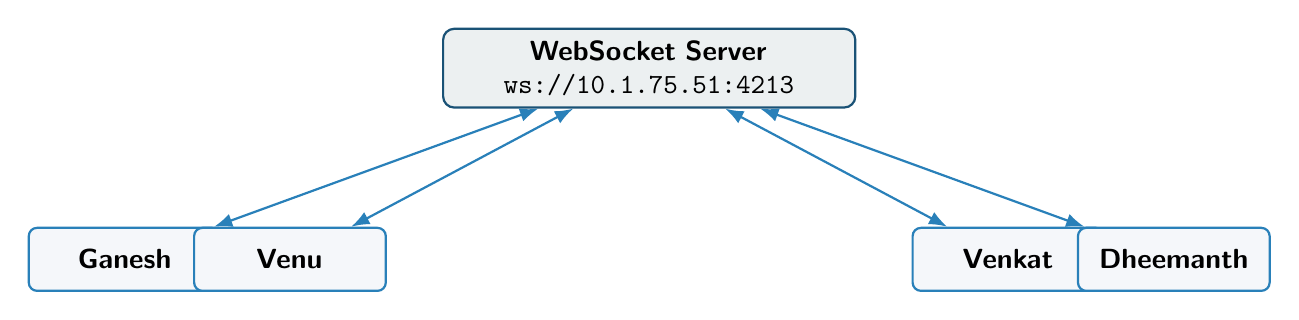
\begin{tikzpicture}[
    serverbox/.style={
        rectangle, draw=primaryblue, fill=codebg, thick,
        text width=5cm, align=center, minimum height=1cm, rounded corners=4pt
    },
    clientbox/.style={
        rectangle, draw=secondaryblue, fill=lightgray, thick,
        text width=2.2cm, align=center, minimum height=0.8cm, rounded corners=3pt
    },
    arrow/.style={<->, >=Latex, thick, color=secondaryblue}
]
    \node [serverbox] (server) {
        \textbf{WebSocket Server}\\
        \texttt{ws://10.1.75.51:4213}
    };

    \node [clientbox, below left=1.5cm and 2.8cm of server]  (c1) {\textbf{Ganesh}};
    \node [clientbox, below left=1.5cm and 0.7cm of server]  (c2) {\textbf{Venu}};
    \node [clientbox, below right=1.5cm and 0.7cm of server] (c3) {\textbf{Venkat}};
    \node [clientbox, below right=1.5cm and 2.8cm of server] (c4) {\textbf{Dheemanth}};

    \draw [arrow] (server) -- (c1);
    \draw [arrow] (server) -- (c2);
    \draw [arrow] (server) -- (c3);
    \draw [arrow] (server) -- (c4);
\end{tikzpicture}
\end{center}

\end{document}
